\section{Inverse Matrix, Basiswechsel}
Ist $A=\begin{pmatrix}a_{1} & b_{1} \\ a_{2} & b_{2} \end{pmatrix}$ und $\lambda \in \mathbb{R}: \ \lambda \cdot A = \begin{pmatrix} \lambda a_{1} & \lambda b_{1} \\ \lambda a_{2} & \lambda b_{2} \end{pmatrix}$\\
%
%
%
\subsubsection{Satz:}
Für $A=\begin{pmatrix}a_{1} & b_{1} \\ a_{2} & b_{2} \end{pmatrix}$ mit $det(A) \neq 0$ gilt:\\
$A^{-1} = \frac{1}{det(a)} \cdot \begin{pmatrix} b_{2} & -b_{1} \\ -a_{2} & a_{1} \end{pmatrix}$
%
%
%
\subsubsection{Beweis:}
$A\cdot A^{-1} = \begin{pmatrix}a_{1} & b_{1} \\ a_{2} & b_{2} \end{pmatrix} \cdot \frac{1}{det(a)} \cdot \begin{pmatrix} b_{2} & -b_{1} \\ -a_{2} & a_{1} \end{pmatrix}$\\
$ = \frac{1}{det(a)} \cdot \begin{pmatrix} det(A) & 0 \\ 0 & det(A) \end{pmatrix}$\\
$= \begin{pmatrix} 1 & 0 \\ 0 & 1 \end{pmatrix}$\\
$A^{-1}\cdot A$ analog $\Rightarrow A^{-1} \cdot A = \begin{pmatrix} 1 & 0 \\ 0 & 1 \end{pmatrix}$ \\
$\mathcal{B} = (\vec{b_{1}}, \vec{b_{2}})$ Basis $ \leadsto \begin{pmatrix} b_{11} & b_{21} \\ b_{12} & b_{22} \end{pmatrix} = B \qquad \vec{b_{1}} = \begin{pmatrix} b_{11} \\ b_{12} \end{pmatrix}, \qquad \vec{b_{2}}=\begin{pmatrix} b_{21} \\ b_{22} \end{pmatrix}$\\
$\vec{a} = x_{1}\vec{b_{1}} + x_{2}\vec{b_{2}} = B\vec{x}  \qquad  :\vec{x} = B^{-1}\vec{a}$\\
Die Koordinaten von $a$ bzgl. $\mathcal{B}$ sind durch $B^{-1}(\vec{a})$ gegeben, denn man muss das Gleichungssystem $x_{1}b_{1}+x_{2}b_{2}=a$ nach $x_{1}$ und $x_{2}$ lösen. \\
$\mathcal{C} := ( c_{1}, c_{2}). \, A$ ist bestimmt durch $A(c_{1})$ und $A(c_{2})$. \\
$A(c_{1}) = d_{11}b_{1}+d_{21}b_{2} \qquad A(c_{2})=d_{12}b_{1}+d_{22}b_{2}$\\
$_{\mathcal{B}}A_{\mathcal{C}} = \begin{pmatrix}d_{11} & d_{21} \\ d_{12} & d_{22} \end{pmatrix}$ Matrix von $A$ bzgl. $\mathcal{B},\, \mathcal{C}$\\
%
%
%
\subsubsection{Satz:}
$\mathcal{B} = (\vec{b_{1}} \vec{b_{2}}) \qquad \mathcal{C} = (\vec{c_{1}}, \vec{c_{2}})$\\
$B$ bzw. $C$ Matrix mit den Spalten $\vec{b_{1}}, \vec{b_{2}}$ bzw. $\vec{c_{1}}, \vec{c_{2}}$ und ist $A: \mathbb{R}^{2} \rightarrow \mathbb{R}^{2}$ linear. Dann gilt:\\
$_{\mathcal{B}}A_{\mathcal{C}}=B^{-1}AC$\\
%
%
%
\subsubsection{Beweis:}
In der ersten Spalte von $C$ steht das Bild $c_{1}$ von $e_{1}$\\
In der ersten Spalte von $AC$ steht das Bild von $c_{1}$ unter $A$\\
In der ersten Spalte von $B^{-1}AC$ stehen die Koordinaten von $A(c_{1})$ bzgl. $\mathcal{B}$ Analog gilt dies für $c_{2}$.
%
%
%
\subsubsection{Beispiel:}
$\mathcal{B}=(b_{1},b_{2}) \quad b_{1}=\begin{pmatrix} 2 \\ 1 \end{pmatrix}, b_{2}=\begin{pmatrix}5 \\ 3\end{pmatrix}$\\
$A$ gegeben durch $\begin{pmatrix} -1 & 0 \\ 0 & 2 \end{pmatrix}$\\
$_{\mathcal{B}}A_{\mathcal{B}}=\begin{pmatrix} 3 & -5 \\ -1 & 2 \end{pmatrix} \mathop{\underbrace{\begin{pmatrix} -1 & 0 \\ 0 & 2\end{pmatrix} \begin{pmatrix}2 & 5 \\ 1 & 3 \end{pmatrix}}}\limits_{\begin{pmatrix}-2 & -5 \\ 3 & 6 \end{pmatrix}}= \begin{pmatrix} -16 & -45 \\ 6 & 17\end{pmatrix}$
%
%
%
\subsubsection{Satz:}
$A,B$ invertierbar $\Rightarrow A \cdot B$ invertierbar, Inverse $B^{-1}A^{-1}$
%
%
%
\subsubsection{Beweis:}
$(AB)(AB)^{-1}=A(BB^{-1})A^{-1}=AEA^{-1}|E=\begin{pmatrix}1 & 0 \\ 0 &1 \end{pmatrix}$\\
$B^{-1}A^{-1}AB=E \, \checkmark$\\
Im Allgemeinen: $E \neq ABA^{-1}B^{-1}$!
%
%
%
\subsubsection{Beispiel:}
$A=\begin{pmatrix} 1 & 12 \\ 2 & 3 \end{pmatrix}$ Frage: Gibt es eine Basis $b_{1}b_{2}: \,  _{\mathcal{B}}A_{\mathcal{B}} = \begin{pmatrix} 7 & 0 \\ 0 & -3 \end{pmatrix}$? \\
Insbesondere $A(b_{1})=7b_{1}$  $\begin{pmatrix}1 & 12 \\ 2 & 3 \end{pmatrix} \begin{pmatrix} x \\ y \end{pmatrix} = \begin{pmatrix} 7x \\ 7y \end{pmatrix}$ \\
$\rightarrow
\begin{array}{rcr}
x + 12y &=& 7x\\
2x + 3y &=& 7y\\
\end{array}
\mathop{\Rightarrow}\limits^{\text{Cramersche}}_{\text{Regel}} b_{1} = \begin{pmatrix} 2 \\ 1 \end{pmatrix}$\\
$A(b_{2}) = -3b_{2} \mathop{\Rightarrow}\limits^{\text{Cramersche}}_{\text{Regel}} b_{2} = \begin{pmatrix} 3 \\ -1 \end{pmatrix}$\\
%
%
%
\subsubsection{Probe:}
$\begin{pmatrix} -1 & -3 \\ -1 & 2 \end{pmatrix} \cdot \begin{pmatrix} 1 & 12 \\ 2 & 3 \end{pmatrix} \begin{pmatrix}2 & 3 \\ 1 & -1 \end{pmatrix} = \frac{1}{5} \begin{pmatrix} 35 & 0 \\ 0 & -15 \end{pmatrix} = \begin{pmatrix} 7 & 0 \\ 0 & -3 \end{pmatrix}$
%
%
%
\subsubsection{Satz:}
Sei $A: \mathbb{R}^{2} \rightarrow \mathbb{R}^{2}$ linear. Dann gibt es Basen $\mathcal{B}, \mathcal{C}$ von $\mathbb{R}^{2}$, sodass $_{\mathcal{B}}A_{\mathcal{C}}$ eine der Formen annimmt $\begin{pmatrix} 1 & 0 \\ 0 & 1 \end{pmatrix}, \begin{pmatrix} 0 & 0 \\ 0 & 0 \end{pmatrix}, \begin{pmatrix} 1 & 0 \\ 0 & 0 \end{pmatrix}$
%
%
%
\subsubsection{Beweis:}
Setze $A\begin{pmatrix} 1 \\ 0 \end{pmatrix} = \vec{a} \qquad A \begin{pmatrix} 0 \\ 1 \end{pmatrix} = \vec{b}$
\begin{enumerate}
	\item $\vec{a} = \begin{pmatrix} 0 \\ 0 \end{pmatrix} = \vec{b} \qquad \mathcal{B} = 
		\mathcal{E} = \mathcal{C} \checkmark$
	\item Wenn $\mathcal{A} = (\vec{a},\vec{b})$ Basis, $\mathcal{C}=\mathcal{E} \qquad 
		\mathcal{B}  = \mathcal{A}$ \\ 
		$_{\mathcal{A}}A_{\mathcal{B}}=A^{-1}A=\begin{pmatrix} 1 & 0 \\ 0 & 1 
		\end{pmatrix}$\\
		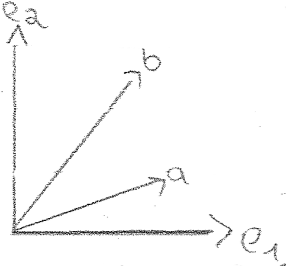
\includegraphics[width=0.2\textwidth]
	{mainmatter/chapter1/pics/grafik13.png}
	\item $\vec{a}, \vec{b}$ keine Basis, aber $\vec{a} \neq \begin{pmatrix} 0 \\ 0 
		\end{pmatrix} \rightarrow \vec{b} = \lambda \vec{a}$ und $A\begin{pmatrix}\lambda	
		\\ -1\end{pmatrix} = \lambda \vec{a} - \vec{b} = \begin{pmatrix} 0 \\ 0 
		\end{pmatrix} \qquad \mathcal{B} = (\vec{a},\vec{a}_{\perp})$\\
		$_{\mathcal{B}}A_{\mathcal{C}} = B^{-1}A\cdot C = \frac{1}{a_{1}^{2}+a_{2}^{2}} 
		\begin{pmatrix} a_{1} & a_{2} \\ -a_{2} & a_{1} \end{pmatrix} 
		\mathop{\underbrace{\begin{pmatrix} a_{1} & b_{1} \\ a_{2} & b_{2} 
		\end{pmatrix} \begin{pmatrix} 1 & \lambda \\ 0 & -1 
		\end{pmatrix}}}\limits_{\begin{pmatrix} a_{1} & 0 \\ a_{2} & 0 
		\end{pmatrix}}=\begin{pmatrix} 1 & 0 \\ 0 & 0 \end{pmatrix}$
\end{enumerate}